%%%%%%%%%%%%%%%%%%%%%%%%%%%%%%%%%%%%%%%%%%%%%%%%%%%%%%%%%%%%%%%%%%%%%%
% Lớp 10 | Hàm số bậc hai và đồ thị | Hàm số bậc hai
% Dạng 0D3?2-2: Bảng biến thiên, tính đơn điệu, max, min
% Số câu: 20  (sinh tự động bởi tach_cau.py; từ nay thầy sửa trực tiếp file này)
%%%%%%%%%%%%%%%%%%%%%%%%%%%%%%%%%%%%%%%%%%%%%%%%%%%%%%%%%%%%%%%%%%%%%%

%%%%%%%%%%%%%%%% TRẮC NGHIỆM 4 PHƯƠNG ÁN %%%%%%%%%%%%%%%%

% nguồn: MaHoaNH_TracNghiem_Lop10
\begin{ex}%[0D3N2-2]%[ma:e5100cdd]
	Trục  đối xứng của parabol $y=3x^2-2x+1$ là đường thẳng
	 \choice
		{$x=-\dfrac{1}{3}$} 
		{$x=\dfrac{2}{3}$} 
		{\True  $x=\dfrac{1}{3}$}
		{$y=\dfrac{1}{3}$} 
	\loigiai{Hàm số  bậc hai có trục đối xứng $x=-\dfrac{b}{2a}=\dfrac{1}{3}$.}
\end{ex}

% nguồn: MaHoaNH_TracNghiem_Lop10
\begin{ex}%[0D3N2-2]%[ma:46aa1020]
	Hàm số $y=x^2-8x+12$ nghịch  biến trên khoảng
	\choice 
		{$(8;+\infty)$} 
		{$(-\infty;8)$} 
		{\True  $(-\infty;4)$}
		{$(4;+\infty)$} 
	 \loigiai{
		 Hàm số $y=x^2-8x+12$ có hệ số $a=1>0$ nên hàm số nghịch biến trên khoảng $\left(-\infty;-\dfrac{b}{2a}\right)$.\\
	Vì vậy hàm số  đã cho nghịch biến trên $(-\infty;4)$.}
\end{ex}

% nguồn: MaHoaNH_TracNghiem_Lop10
\begin{ex}%[0D3N2-2]%[ma:23d55c1b]
	Cho parabol có phương  trình $y=x^2-3x+2$. Xác định hoành độ đỉnh của Parabol.
	 \choice
		{$x=-3$} 
		{$x=-\dfrac{3}{4}$} 
		{$x=-\dfrac{3}{2}$} 
		 {\True $x=\dfrac{3}{2}$}
	\loigiai{Hoành độ đỉnh của parabol $y=ax^2+bx+c$ là  $x=-\dfrac{b}{2a}$.\\
		Trong phương trình $y=x^2-3x+2$, ta có $a=1, b=-3,  c=2$.\\
	Vậy hoành độ đỉnh của parabol là $x=-\dfrac{-3}{2\cdot(1)} =  \dfrac{3}{2}$.}
\end{ex}

% nguồn: MaHoaNH_TracNghiem_Lop10
\begin{ex}%[0D3H2-2]%[ma:ff926336]
	Cho parabol $(P)\colon  y=3x^2-2x+1$. Điểm nào sau đây là đỉnh của $(P)$?
	 \choice
		{\True $I\left(\dfrac{1}{3};\dfrac{2}{3}\right)$} 
		 {$I(0;1)$}
		{$I\left(-\dfrac{1}{3};\dfrac{2}{3}\right)$} 
		{$I\left(\dfrac{1}{3};-\dfrac{2}{3}\right)$} 
	 \loigiai{
		Xét $(P)\colon  y=3x^2-2x+1$, ta có $a=3$; $b=-2$; $c=1$.\\
		Suy ra $x=-\dfrac{b}{2a}=\dfrac{1}{3}\Rightarrow y=\dfrac{2}{3}$.\\ 
		Vậy đỉnh  của $(P)$ là $I\left(\dfrac{1}{3};\dfrac{2}{3}\right)$.
	 }
\end{ex}

% nguồn: MaHoaNH_TracNghiem_Lop10
\begin{ex}%[0D3H2-2]%[ma:d77c4847]
	Xác định parabol $(P)\colon y=a  x^2+b x+c$ biết $(P)$ có giá trị lớn nhất bằng $3$ tại $x=2$ và cắt trục $O x$ tại điểm có hoành độ bằng $1$.
	\choice 
		{$y=-x^2+4x-3$} 
		{$y=x^2-4x+7$} 
		 {$y=2x^2-12x+20$}
		{\True $y=-3x^2+12x-9$} 
	 \loigiai{
		 Vì $(P)$ có giá trị lớn nhất bằng $3$ tại $x=2$ nên $(2; 3)$ là tọa độ đỉnh của parabol và $a<0$.\\
		Do đó $\heva{&\dfrac{-b}{2 a}=2\\&4 a+2b+c=3}$.\\ 
		Vì $(P)$ cắt  trục $O x$ tại điểm có hoành độ bằng $1$ nên $a+b+c=0$.\\
		Do  đó $a=-3$, $b=12$, $c=-9$.
	 }
\end{ex}

% nguồn: MaHoaNH_TracNghiem_Lop10
\begin{ex}%[0D3H2-2]%[ma:d7a51d66]
	Hàm số $y=x^2-4x+11$ đồng biến  trên khoảng nào trong các khoảng sau đây?
	 \choice
		 {$(-2;+\infty)$}
		{$(-\infty;+\infty)$} 
		 {\True$(2;+\infty)$}
		{$(-\infty;2)$} 
	\loigiai{ 
		Ta có  bảng biến thiên
		\begin{center}
			\begin{tikzpicture}
					\tkzTabInit[nocadre=true,lgt=1,espcl=2.5,deltacl=0.5] 
						 {$x$/0.7,$y$/2}
						 {$-\infty$,$2$,$+\infty$}
					 \tkzTabVar{+/$+\infty$,-/$7$,+/$+\infty$}
				\end{tikzpicture}
		\end{center}
		Từ  bảng biến thiên ta thấy, hàm số đồng biến trên khoảng $(2;+\infty)$.
	} 
\end{ex}

% nguồn: MaHoaNH_TracNghiem_Lop10
\begin{ex}%[0D3H2-2]%[ma:0225e689]
	 \immini[thm]{
	 Hàm số nào có bảng biến thiên như hình đưới đây?
	\choice 
		{$y=-x^2+4x-3$} 
		 {$y=2x^2-8x+7$}
		 {\True$y=x^2-4x+5$}
		 {$y=\dfrac{1}{2}x^2-2x+1$}
		 }{
		\begin{tikzpicture}
				\tkzTabInit[nocadre=true,lgt=1,espcl=2.5,deltacl=0.5] 
					{$x$/0.7,$y$/2} 
					{$-\infty$,$2$,$+\infty$} 
				 \tkzTabVar{+/$+\infty$,-/$1$,+/$+\infty$}
			\end{tikzpicture}
		 }
	 \loigiai{
		Từ bảng biến  thiên ta loại $y=-x^2+4x-3$.\\
		Gọi $A\left(x_A; y_A\right)$ là đỉnh của  parabol, ta có:
		$\heva{&x_A=2\\&y_A=1}$.\\ 
		Suy  ra ta loại $y=2 x^2-8 x+7$ và $y=\dfrac{1}{2}x^2-2x+1$.
	} 
\end{ex}

% nguồn: MaHoaNH_TracNghiem_Lop10
\begin{ex}%[0D3Y2-2]%[ma:49f74143]
	Bảng xét dấu 
	\begin{center}
		\begin{tikzpicture}
				 \tkzTabInit[nocadre=false,lgt=1.1,espcl=1.8,deltacl=0.5]
					 {$x$/.7,$f (x)$/.7}
					 {$-\infty$,$1$,$3$,$+\infty$}
				\tkzTabLine{,-,$0$,+,$0$,-} 
			\end{tikzpicture}
	\end{center}
	là của tam thức bậc hai nào dưới đây? 
	\choice 
		 {\True $f(x)=-x^2 +4x -3$}
		{$f(x)=x^2  -4x +3$}
		{$f(x)=-x^2  +x -3$}
		{$f(x)=-x^2  +4x $}
	\loigiai{Từ bảng xét dấu suy ra hệ số $a<0$, nghiệm của biểu thức là $x=1$ hoặc $x=3$. Do đó $f(x)=-x^2 +4x -3$. 
	} 
\end{ex}

% nguồn: MaHoaNH_TracNghiem_Lop10
\begin{ex}%[0D3B2-2]%[ma:d3f91c62]
	\immini{ 
	Bảng biến thiên như hình bên là  bảng biến thiên của hàm số nào?
	\choice 
		 {\True $y=x^2+2x-2$}
		 {$y=x^2-2x-2$}
		 {$y=-x^2-2x-2$}
		 {$y=x^2+3x-2$}}
		{\vspace{-0.5cm} 
		\begin{tikzpicture}
				\tkzTabInit[nocadre=true,lgt=1.2,espcl=2.5,deltacl=0.6] 
					 {$x$/0.6,$y$/2}
					{$-\infty$,$-1$,$+\infty$} 
				 \tkzTabVar{+/$+\infty$,-/$-3$,+/$+\infty$}
			\end{tikzpicture}
		 }
	 \loigiai{
		Bảng biến thiên  thể hiện đồ thị hàm số có bề lõm quay lên nên $a>0$.\\
		Hoành độ đỉnh parabol là $x=-1$.\\ 
		Trong $4$ hàm số  được cung cấp, chỉ có $y=x^2+2x-2$ có tính chất như thế.
	} 
\end{ex}

% nguồn: MaHoaNH_TracNghiem_Lop10
\begin{ex}%[0D3Y2-2]%[ma:8f2e1c04]
	 \immini{
	Cho hàm  số $y=f(x)=ax^2+bx+c$ có đồ thị như hình vẽ.
	 Hàm số $f(x)<0$ với mọi $x$ thuộc khoảng?
	 \choice
		{$\left(4;5\right)$} 
		{$\left(-1;4\right)$} 
		{$\left(0;1\right)$} 
		{\True $\left(1;4\right)$}} 
		{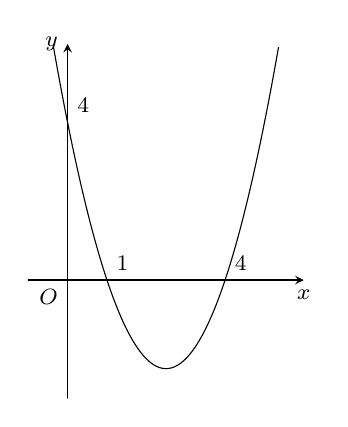
\begin{tikzpicture}[scale=.5,>=stealth,font=\footnotesize,line join=round,line cap=round]
		\def\a{1} \def\b{-5}  \def\c{4}
		 \def\xmin{-1} \def\xmax{6}
		\def\ymin{-3} \def\ymax{6} 
		\draw[->] (\xmin,0)--(\xmax,0)  node [below]{$x$};
		\draw[->]  (0,\ymin)--(0,\ymax) node [left]{$y$};
		\node at  (0,0) [below left]{$O$};
		 \draw (1,0) node[above right] {$1$};
		\draw (4,0) node[above right] {$4$}; 
		\draw (0,4) node[above right]  {$4$};
		\clip (\xmin+0.1,\ymin+0.1) rectangle  (\xmax-0.5,\ymax-0.1);
		\draw[smooth,samples=300][domain=-1:6] plot  (\x,{\a*(\x)^2+\b*(\x)+\c});
	\end{tikzpicture}
		} 
	\loigiai{Dựa vào đồ thị  ta có $f(x)<0\Leftrightarrow x\in\left(1;4\right)$
	 }
\end{ex}

% nguồn: MaHoaNH_TracNghiem_Lop10
\begin{ex}%[0D3Y2-2]%[ma:91240ccd]
	 \immini{
	Cho hàm bậc hai  $y=ax^2+bx+c$, $a\neq 0$ có đồ thị như hình vẽ dưới đây.
	Hàm số đã cho đồng biến trên khoảng nào sau  đây?
	\choice 
		 {$(-\infty;-1)$}
		 {$(-2;+\infty)$}
		{\True $(-1;+\infty)$} 
		 {$(-\infty;0)$}
		 }
		{ 
		\begin{tikzpicture}[line cap=butt,line join=miter,>=stealth]
				\tikzset{declare function={xmin=-3; xmax=2; ymin=-2.5; ymax=2; 
					 f (\x)=1*(\x)^2+2*(\x)-1;
					}, 
					 smooth,samples=450
				} 
				\draw[->] (xmin,0)--(xmax,0) node[shift={(-100:7pt)},font=\normalsize]{$ x  $};
				\draw[->] (0,ymin)--(0,ymax) node[shift={(190:7pt)},font=\normalsize]{$ y $}; 
				 \fill (0,0) node[shift={(225:7pt)},font=\normalsize]{$ O $};
				\draw[dashed]  (-2,0) node[above]{$-2$}
					 (-1,0) node[above]{$-1$}--(-1,-2)--(0,-2) node[right]{$-2$}
					(0,-1)  node[right]{$-1$};
				\fill (-1,-2)  circle (1pt); \fill (-2,0) circle (1pt); \fill (0,-1) circle (1pt);
				\clip (xmin,ymin) rectangle  (xmax,ymax);
				\draw plot[domain=xmin:xmax] (\x,{f (\x)}); 
			\end{tikzpicture}
		} 
	\loigiai{ 
		Hàm số đã cho đồng biến trên  khoảng $(-1;+\infty)$.
	 }
\end{ex}


%%%%%%%%%%%%%%%% ĐÚNG/SAI %%%%%%%%%%%%%%%%

% nguồn: MaHoaNH_DungSai_Lop10
\begin{ex}%[0D3N2-2]%[ma:4957d7b6]
	Cho hàm số $y=  2x^2-4x+1$. Các khẳng định sau đây đúng hay sai?
	 \choiceTF
		 {Hàm số đồng biến trên $(0;+\infty)$}
		{Hàm số nghịch biến trên $(-\infty; 2)$} 
		{\True Hàm số  đồng biến trên $(2;+\infty)$}
		 {\True Hàm số nghịch biến trên $(-\infty;0)$}
	 \loigiai{
		Ta có $a=2 >0$; $-\dfrac{b}{2a} =1$, nên hàm  số
		\begin{itemize}
			\item Hàm số đồng biến  trên $(1;+\infty)$;
			\item Hàm số nghịch biến  trên $(-\infty;1)$.
		\end{itemize}
		Suy  ra
		\begin{itemchoice}
			\itemch Hàm  số không đồng biến trên $(0;+\infty)$.
			 \itemch Hàm số không nghịch biến trên $(-\infty; 2)$.
			 \itemch Hàm số đồng biến trên $(2;+\infty) \subset (1;+\infty)$.
			\itemch Hàm số nghịch  biến trên $(-\infty;0) \subset (-\infty;1)$.
		\end{itemchoice}
	} 
\end{ex}

% nguồn: MaHoaNH_DungSai_Lop10
\begin{ex}%[0D3H2-2]%[ma:a52b47fa]
	 Cho hàm số $y =-x^2+6x+2$. Các khẳng định sau đây đúng hay sai?
	 \choiceTF
		{Hàm số đạt giá trị nhỏ nhất bằng  $-11$}
		{\True Hàm số đồng biến trên $(-\infty;3)$} 
		{\True Hàm số đạt giá trị lớn  nhất bằng $11$}
		{Hàm số nghịch biến  trên $(0;+\infty)$}
	\loigiai{ 
		\begin{itemchoice}
			\itemch  Hàm số đạt giá trị lớn nhất bằng $11$ tại $x=3$.
			 \itemch Hàm số đồng biến trên $(-\infty;3)$.
			\itemch Hàm số nghịch biến trên  $(3;+\infty)$.
		\end{itemchoice}
	 }
\end{ex}

% nguồn: MaHoaNH_DungSai_Lop10
\begin{ex}%[0D3H2-2]%[ma:9736ab6c]
	Cho hàm số $f(x) = -2x^2+ mx +4$ ($m$ là tham  số).
	Các khẳng định sau đây đúng hay sai? 
	 \choiceTF
		{\True Hàm  số không đồng biến trên $(-\infty; +\infty)$ với mọi $m$}
		{\True Không tồn tại giá trị  của $m$ để hàm số không đồng biến trên $(0;+\infty)$}
		{Hàm số nghịch biến trên $(-1;+\infty)$ khi và chỉ khi  $m \leq 4$}
		{\True  Hàm số đồng biến trên $(-\infty;0)$ khi và chỉ khi $m \geq 0$}
	\loigiai{ 
		Ta có  $a=-2<0$; $-\dfrac{b}{2a} =\dfrac{m}{4}$, nên hàm số $f(x)$
		\begin{itemize}
			 \item Hàm số đồng biến trên $\left(-\infty;\dfrac{m}{4}\right)$;
			\item  Hàm số nghịch biến trên $\left(\dfrac{m}{4}; +\infty \right)$.
		\end{itemize}
		\begin{itemchoice}
			\itemch Hàm số  $f(x) $ là hàm số bậc hai nên không đồng biến trên $(-\infty; +\infty)$ với mọi $m$.
			\itemch Hàm số $f(x)$ là hàm số bậc hai có hệ số $a<-1$ nên hàm số không  đồng biến trên $(0;+\infty)$
			\itemch Hàm số nghịch biến trên $(-1;+\infty)$ khi và chỉ khi $\dfrac{m}{4} \leq -1 \Leftrightarrow  m \leq -4$.
			\itemch Hàm số đồng biến trên $(-\infty;0)$ khi  và chỉ khi $\dfrac{m}{4} \geq 0 \Leftrightarrow m \geq 0$.
		\end{itemchoice}
	 }
\end{ex}

% nguồn: MaHoaNH_DungSai_Lop10
\begin{ex}%[0D3H2-2]%[ma:357a30a0]
	Cho hàm số bậc hai có  bảng biến thiên
	\begin{center}
		\begin{tikzpicture}
				 \tkzTabInit[lgt=1.5,espcl=2.5,deltacl=.5]
					{$x$ /.7,$y$  /2}
					{$+\infty$,$-1$,$+\infty$} 
				 \tkzTabVar{+/$+\infty$,-/ $2$,+/$+\infty$}
			\end{tikzpicture}
	\end{center}
	Các khẳng định sau đây  đúng hay sai?
	 \choiceTF
		{\True Hàm số đồng biến trên $(-1;+\infty)$} 
		{\True Hàm số đạt giá trị nhỏ  nhất bằng $2$}
		{Hàm  số nghịch biến trên $(-\infty;2)$}
		{Hàm  số đạt giá trị nhỏ nhất tại $x=2$}
	\loigiai{ 
		\begin{itemchoice}
			\itemch Hàm số đồng  biến trên $(-1;+\infty)$.
			\itemch Hàm số nghịch  biến trên $(-\infty;-1)$.
			\itemch Hàm số đạt giá trị nhỏ nhất  bằng $2$ tại $x=-1$.
		\end{itemchoice}
	 }
\end{ex}

% nguồn: MaHoaNH_DungSai_Lop10
\begin{ex}%[0D3H2-2]%[ma:c724474c]
	Cho hàm số bậc hai $y= f(x)$ có  $f(2) = 2$ và bảng biến thiên
	\begin{center}
		\begin{tikzpicture}
				 \tkzTabInit[lgt=1.5,espcl=2.5,deltacl=.5]
					{$x$  /.7,$f (x)$ /2}
					 {$-\infty$,$1$,$-\infty$}
				\tkzTabVar{-/$-\infty$,+/ $3$,-/$-\infty$} 
			\end{tikzpicture}
	\end{center}
	Các khẳng định sau đây  đúng hay sai?
	\choiceTF 
		{\True Hàm số  đạt giá trị lớn nhất bằng $3$}
		{Hàm số bậc hai là $y= -2x^2+4x+2$} 
		{\True  Giá trị của hàm số tại $x=0$ là $2$}
		{\True Giá trị của hàm số tại $x=-1$ là $-1$} 
	\loigiai{ 
		\begin{itemchoice}
			\itemch Hàm số đạt giá trị lớn nhất bằng $3$. 
			 \itemch Gọi $f(x) = ax^2+bx+c$. Từ giả thiết ta có
			\[ 
			 \heva{&4a+2b+c =2\\& 2a+b=0\\&a+b+c =3} \Leftrightarrow \heva{&a=-1\\&b=2\\&c=2.}
			 \]
			 Do đó $f(x) = -x^2+2x+2$.
			\itemch  $f(0)=2$.
			\itemch  $f(-1) =-1$.
		\end{itemchoice}
	 }
\end{ex}


%%%%%%%%%%%%%%%% TRẢ LỜI NGẮN %%%%%%%%%%%%%%%%

% nguồn: MaHoaNH_TraLoiNgan_Lop10
\begin{bt}%[0D3H2-2]%[ma:687e2956]
	Tìm giá trị lớn nhất của hàm số $y=-2x^2+x+5$. Kết quả  làm tròn đến hàng phần mười.
	 \shortans{0,3}
	 \loigiai{
		Xét  hàm số $y=-2x^2+x+5$ có $a=-2< 0$ và có đỉnh $I\left(\dfrac{1}{4}; \dfrac{41}{8}\right)$.\\
		Do đó,  hàm số đạt giá trị lớn nhất bằng $\dfrac{41}{8}$ tại $x=\dfrac{1}{4}\approx0{,}3$.
	} 
\end{bt}

% nguồn: MaHoaNH_TraLoiNgan_Lop10
\begin{bt}%[0D3V2-2]%[ma:cc025c3b]
	Một khách sạn có $50$ phòng. Hiện tại mỗi phòng cho thuê với giá $400$ nghìn đồng mỗi ngày thì toàn bộ phòng đều được thuê. Biết rằng cứ mỗi lần tăng giá thuê $20$ nghìn đồng  thì có thêm $2$ phòng trống. Hỏi nhà đầu tư cần chọn giá phòng nhiều nhất để tổng doanh thu của khách sạn đạt tối đa? (đơn vị: nghìn đồng).
	\shortans{450} 
	 \loigiai{
		 Gọi $x$ (nghìn đồng) là số tiền tăng lên của mỗi phòng. \\
		Giá mỗi phòng sau khi tăng là: $400 + x$ (nghìn đồng).  \\
		Do cứ mỗi lần tăng giá thêm $20$ nghìn đồng thì có thêm  $2$ phòng trống, nên nếu tăng lên $x$ nghìn đồng thì có $\dfrac{x}{10}$ phòng trống.\\
		Số phòng  cho thuê lúc này là $50 - \dfrac{x}{10}$. \\
		Số tiền phòng thu được  lúc này là \\
		$$y = \left(50 -  \dfrac{x}{10}\right)\left(400 + x\right) = \dfrac{1}{10} x^2 + 10x - 20\,000 = -\dfrac{1}{10} (x - 50)^2 + 20\, 250 \leq 20\, 250.$$
		Đặt \lq\lq$=$\rq\rq~xảy ra khi  $x = 50$. \\
		Vậy giá mỗi phòng  là $450$ nghìn đồng mỗi phòng thì lợi nhuận thu được là cao nhất.
	} 
\end{bt}

% nguồn: MaHoaNH_TraLoiNgan_Lop10
\begin{bt}%[0D3V2-2]%[ma:bb79a8ef]
	Một người dân phải chèo thuyền từ vị trí $A$ đến vị trí $C$ trên bờ $BD$, sau đó chạy bộ từ $C$ đến $B$. Biết rằng vận tốc chèo thuyền bằng $6$ km/h, vận tốc chạy bộ là $8$ km/h, khoảng cách từ vị trí $A$ đến bờ $BD$ bằng $3$ km/h, khoảng cách hai vị trí $B, D$ bằng $8$ km. Tính khoảng cách (đơn vị km) lớn nhất giữa hai vị trí $B$ và $C$ biết  rằng tổng thời gian người đó chèo thuyền và chạy bộ là $1$ giờ $20$ phút (kết quả làm tròn đến hàng phần trăm).
	\begin{center}
		\begin{tikzpicture}
				\coordinate (A) at  (0,0);
				\coordinate (D)  at (0,3);
				\coordinate (B)  at (8,3);
				\coordinate (C) at (3,3); 
				\coordinate (E)  at (8,0);
				 \fill[pattern=dots] (A) -- (D) -- (B) -- (E) -- cycle;
				\draw[thick] (A) -- (D) -- (B)  -- (E) -- cycle;
				\draw[thick] (A) --  (C);
				\foreach \point/\label/\position in {A/A/below left,D/D/above  left,B/B/above right,C/C/above,E/ /below right}{
					\node[\position] at (\point) {$\label$}; 
				} 
				 \node at (4,1.5) {con sông};
				\node[rotate=90] at  (-0.3,1.5) {$3$ km};
				\node at  (4,-0.3) {$8$ km};
			\end{tikzpicture}
	\end{center}
	\shortans{5,14} 
	 \loigiai{
		Gọi  thời gian chạy bộ đoạn $BC$ là $x$ giờ $\left(0 < x \leq \dfrac{4}{3}\right)$.\\
		Thời gian chèo thuyền đoạn $AC$ là $\dfrac{4}{3} -  x$ (giờ). \\
		Khi đó quãng đường đoạn $BC$ là $8x$ km, $AC = \left(\dfrac{4}{3} - x\right) \cdot  6$ (km). \\
		Ta tính được  $DC = \sqrt{36 \left(\dfrac{4}{3} - x\right)^2 - 9}$ (km). \\
		Theo giả thiết quãng đường đoạn $BD = 8$ (km) nên  ta có phương trình: \\
		\begin{eqnarray*}
			&& 8x + \sqrt{36 \left(\dfrac{4}{3}  - x\right)^2 - 9} = 8\\
			&\Leftrightarrow&\sqrt{36 \left(\dfrac{4}{3} - x\right)^2  - 9} = 8 - 8x\\
			&\Leftrightarrow&\heva{&x\leq 1\\ & 28x^2 - 32x +  9 =0}\\
			&\Leftrightarrow&\heva{&x\leq 1\\ & \hoac{&  x = \dfrac{1}{2}\\ & x = \dfrac{9}{14}}}\\
			&\Leftrightarrow&\hoac{&x  = \dfrac{1}{2}\\ & x = \dfrac{9}{14}.}
		\end{eqnarray*}
		Với $x =  \dfrac{1}{2}$ giờ, quãng đường $BC = 4$ (km). \\
		Với $x = \dfrac{9}{14}$ giờ, quãng đường $BC = \dfrac{36}{7} \approx 5{,}14$ (km). \\ 
		 Vậy khoảng cách (đơn vị km) lớn nhất giữa hai vị trí $B$ và $C$ bằng $5{,}14$ km.
	 }
\end{bt}


%%%%%%%%%%%%%%%% TỰ LUẬN %%%%%%%%%%%%%%%%

% nguồn: MaHoaNH_TuLuan_Lop10
\begin{bt}%[0D3H2-2]%[ma:6641be9d]
	Cho hàm số  $y=f(x)=-x^2+3$ có đồ thị $(P)$.
	\begin{listEX}
		\item Xét tính đơn điệu của hàm  số $y=f(x)$.
		\item Xác định giá trị lớn nhất của hàm số $y=f(x)$. 
	\end{listEX}
	 \loigiai{
		\begin{listEX}
			 \item Hoành độ đỉnh $x=-\dfrac{b}{2a}=-\dfrac{0}{-2}=0\Rightarrow y=-0^2+3=3$.\\
			Tọa  độ đỉnh $I(0;3)$.\\
			 Ta có bảng biến thiên
			\begin{center}
				\begin{tikzpicture}
						\tkzTabInit[espcl=2.5,lgt=1.5] 
						{$x$/0.7,$y$/2.1} 
						{$-\infty$,$0$,$+\infty$} 
						\tkzTabVar{-/$-\infty$,+/$3$,-/$-\infty$} 
					\end{tikzpicture}
			\end{center}
			Vậy  hàm số đã cho đồng biến trên khoảng $(-\infty;0)$ và nghịch biến trên khoảng $(0;+\infty)$.
			 \item Từ bảng biên thiên ta thấy $y_{\max}=3$ khi $x=0$.
		\end{listEX}
	} 
\end{bt}
